\subsubsection{Projeto de robôs em trilhos}\label{proj_rail}
 % attach a rail to the blade and move it manually
 
 % attach a rail one the nose and ground, 1D movement and move the blade to
A utlização de um manipulador robótico sobre trilhos tem a
capacidade de satisfazer todos os requisitos, até agora observados, para a realização de um
processo de inspeção e metalização utilizando a técnica HVOF. O desenvolvimento
de um sistema compacto para o transporte através dos dutos de acesso e instalção
no camara da turbina é possível, pois o tamanho necessário do manipulador pode
ser reduzido por meio da mobilidade extra proporcionada pela introdução do
trilho.

No contexto da aplicação proposta foram concebidas duas possibilidades para a
fixação do sistema de trilhos. A primeira solução consiste em um sistema
semelhante ao Roboturb, apresentado na seção \ref{sec::rail}. O sistema proposto
se trata de um manipulador robótico, com fixação diretamente na própria pá da
turbina. O trilho deverá ser flexível para ser capaz de acompanhar a curvatura
da pá e possibilitar diversas opções de posicionamento. Como o material da pá
não possui alta permeabilidade magnética (Inox 420), a solução de fixação seria
por ventosas ativas e com material específico para suportar as grandes
variações de temperatura que a pá pode alcançar (temperatura ambiente a
$100^oC$ durante a metalização).

Uma abrangente pesquisa de robôs comerciais industriais de pequeno porte mostrou
que os manipuladores com payload (entre 12 e 20 kg) e velocidade necessários
possuem alcance máximo de 820 mm (LRB da Kuka). A metalização deverá ser
realizada em, pelo menos, quatro etapas com quatro trilhos diferentes e
customizados, e placas de sacrifício deverão ser fixadas durante o
processo para evitar mau aplicação da metalização durante as trocas de sentido
na movimentação do robô. 

A fixação de um trilho na pá apresenta diversas complexidades, como: a
necessidade de manualmente instalar/desinstalar o sistema trilho/robô oito vezes
em cada pá; o projeto do trilho customizado e flexível; e ventosas ativas
especiais que suportam variação de temperatura.

A alternativa para se evitar o contato com a pá consiste em um único trilho
retilíneo fixado por bases magnéticas no solo do aro câmara. Como o robô não
tem alcance de toda a pá, há, ainda, a necessidade de três posições verticais
diferentes. A pá pode ser processada em diagonal, e, neste caso, o manipulador
ficará responsável pela velocidade, posição e orientação do processo. Ou processada na
direção do trilho, e, neste caso, este ficará responsável pela velocidade e o
manipulador fará controle de posição e orientação. Neste último, a troca de
sentido de movimento ocorrerá fora da pá, o que resulta na ausência de placas de
sacrifício. A figura~\ref{rail2} mostra o trilho externo à pá e com
processamento diagonal.

\begin{figure}[h!]
\centering
	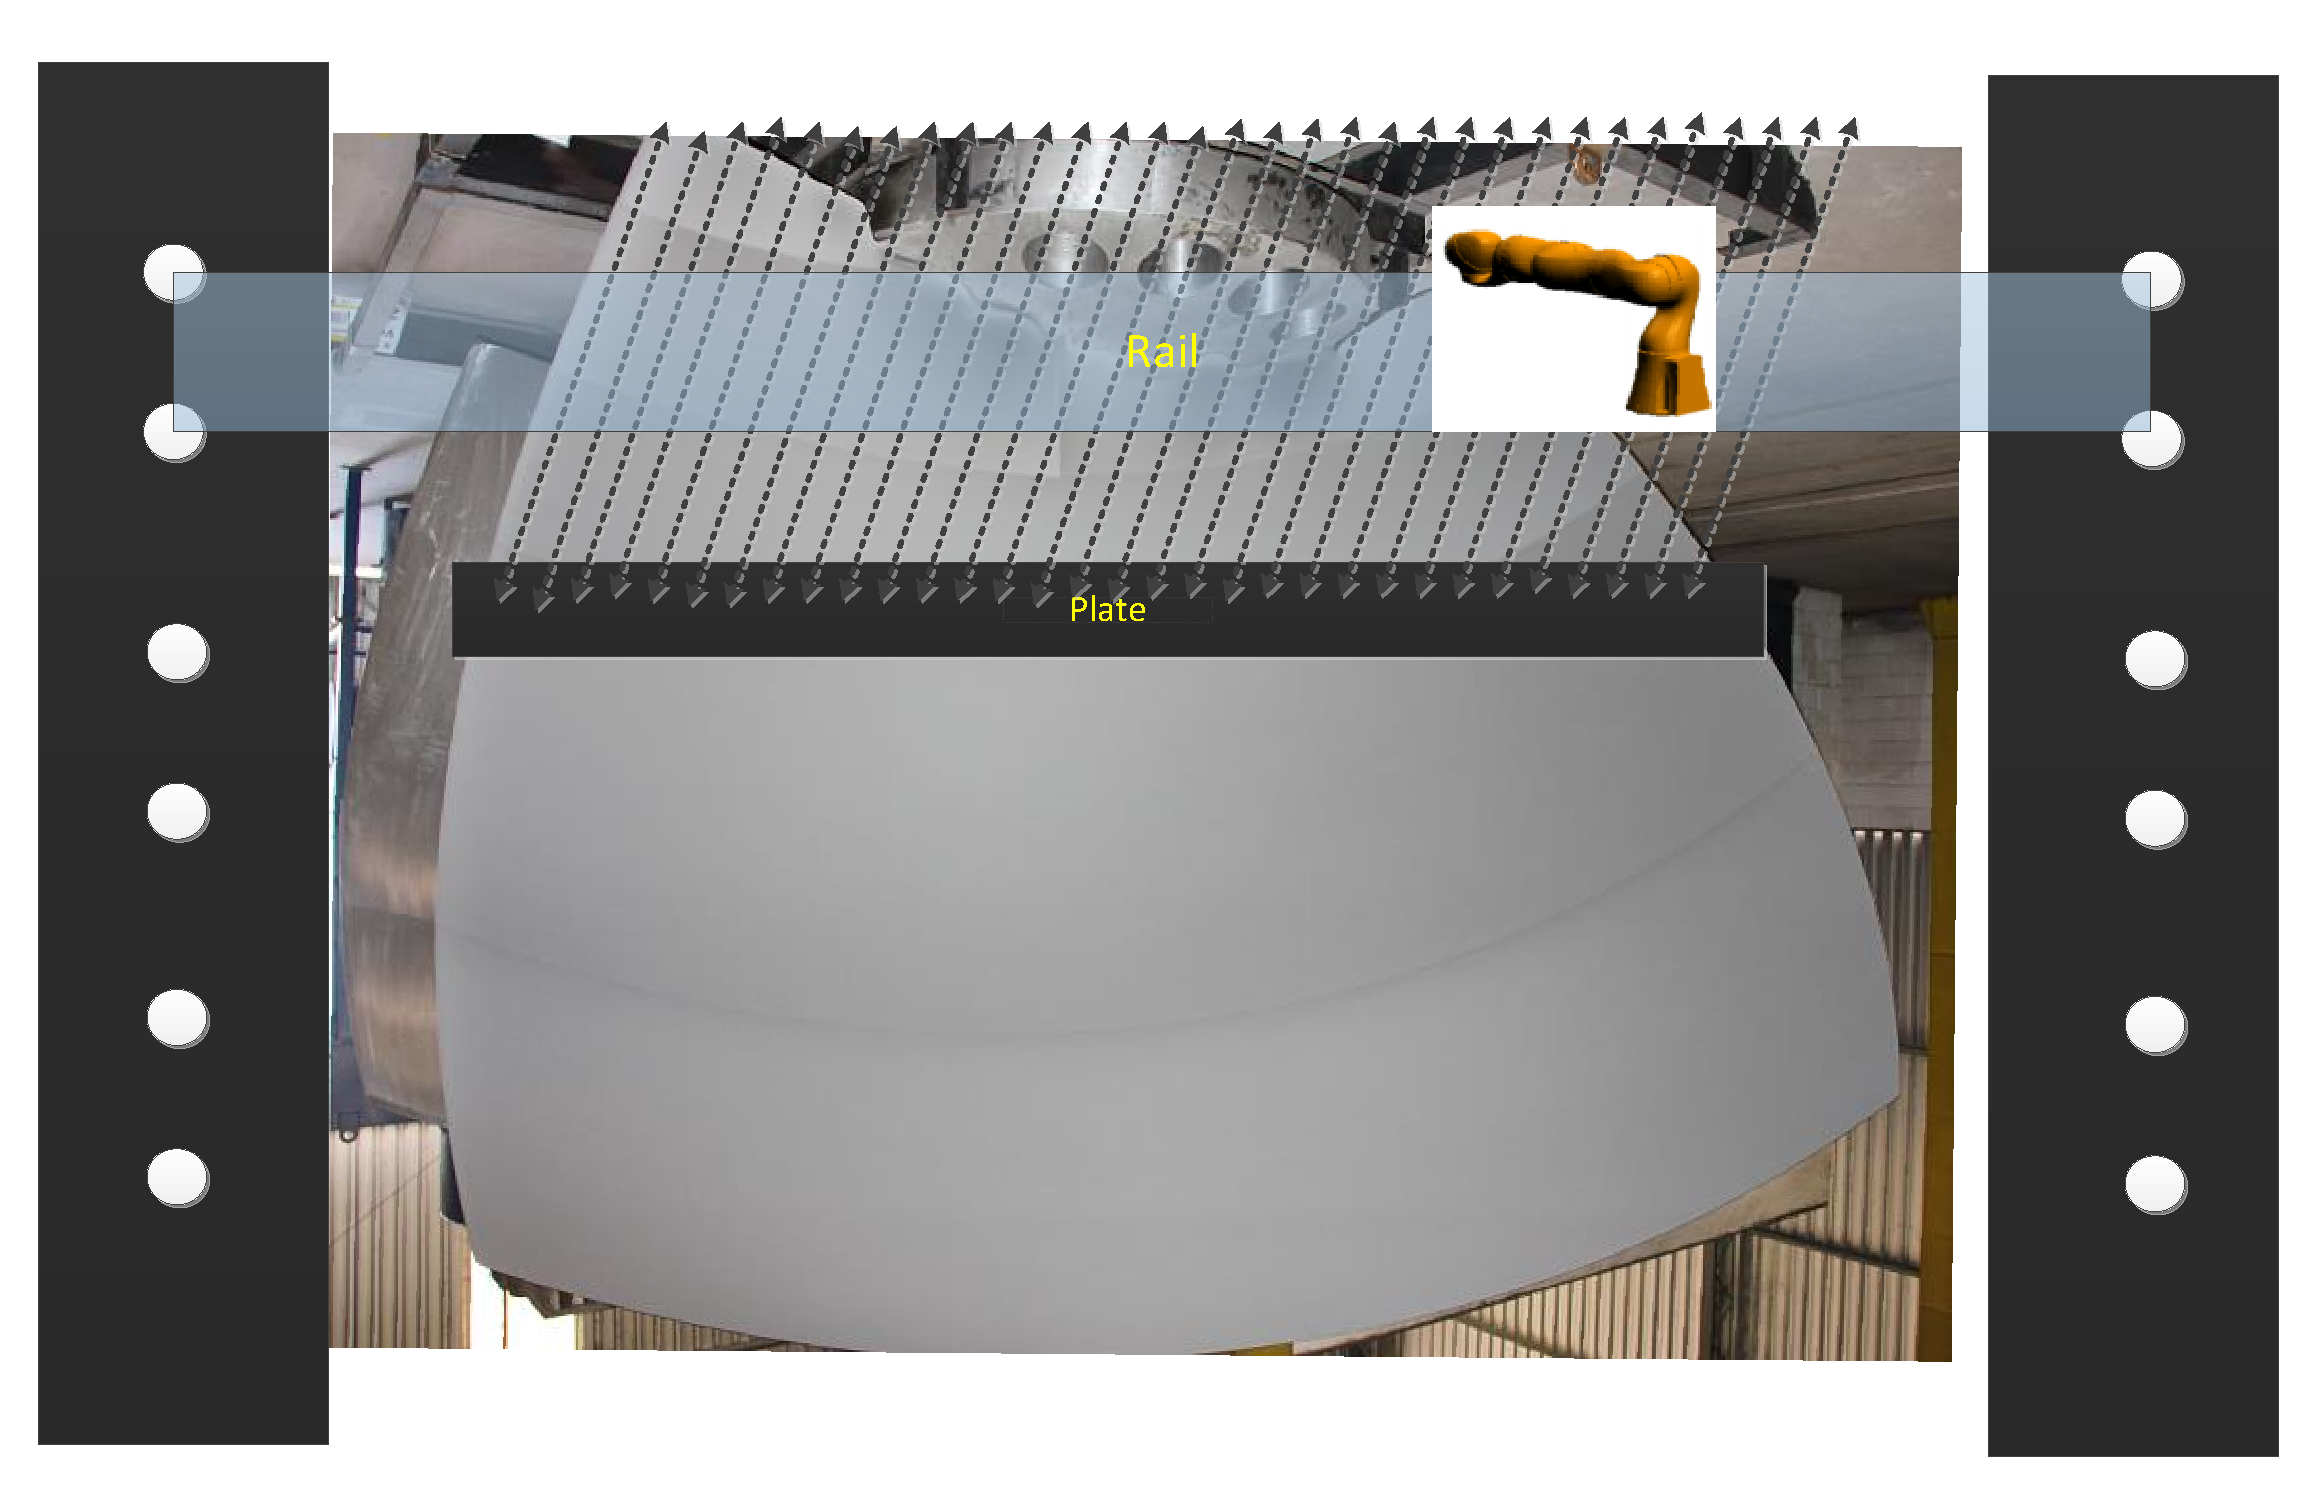
\includegraphics[width=\columnwidth]{figs/trilhos/rail2.pdf}
	\caption{Trilho fora da pá com processamento em diagonal.}
	\label{rail2}
\end{figure}

Esse tipo de abordagem simplifica a movimentação do robô no
trilho, uma vez que o trilho seria totalmente reto, e possibilitaria a
metalização de um dos lados das quatro pás com uma única instalação de base.
Porém, mesmo nesta solução, a altura do trilho deverá ser ajustada três vezes para
cada lado de pá, e toda a estrutura deverá ser reinstalada no outro lado da
turbina para a realização do processo no outro lado das pás.

Em ambos os sistemas propostos, é necessária a implementação de um sistema de
localização do robô em relação à pá, tornando possível a geração de um
planejamento de trajetórias para o processo de metalização. O sistema de
localização pode ser concebido por sensores externos
ao robô (câmeras e outros), ou instalados no próprio manipulador/base.

\textbf{Conclusão da solução por robôs em trilhos}
A solução com trilho externo se mostrou vantajosa em comparação ao robô em
trilho customizado acoplado à pá, devido à complexidade e intervenções
manuais. Há a possibilidade de utilizar um manipulador industrial, sendo
todo o projeto com foco no processamento dos sinais, mapeamento, localização e
controle, além da construção do trilho. Porém, a montagem da estrutura e
instalação de todo o sistema atrás da pá podem ser custosas, sendo esta ainda
uma solução considerada complexa
